\documentclass[a4paper]{article}
\usepackage[utf8]{inputenc}
\usepackage{fullpage}
\usepackage{biblatex}
\bibliography{expose.bib}
\usepackage{graphicx}
\title{Concept for a game prototype}
\author{Willi Schönborn}
\date{\today}
\begin{document}
\maketitle

\section*{Introduction}
The course \textit{Computer Graphics and Effects} (summer term 2011) at the \textit{Beuth Hochschule für Technik Berlin} contains a project assignment to build a game prototype using the jVR rendering framework. The purpose of this document is to explain the ideas and concepts for that game prototype.

\section*{Game Adaptation}
The idea is a partial port of a 2D arcade space shooter game available for mobile devices. The game is called PewPew and is currently available for free for the iPhone and Android platforms.

\begin{figure}[htbp]
\centering
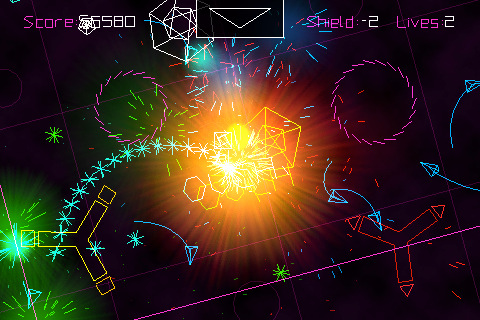
\includegraphics[width=0.75\textwidth]{PewPew-iPhone-App-Review.jpg}
\caption{Visual appearance}
\end{figure}

PewPew ships with several different game modes, levels and enemy types. The core game concept is extremely simple though: The Player has two virtual joysticks which can be used to control the movement of the ship and the direction of the fire. Despite the fact that the game has several game modes, it usually boils down to avoiding collisions and destroying enemies with the ship's gun. The game uses extremely simple vector and wireframe graphics extensively with the effect of a very harmonious visual appearance.

\newpage

\section*{Ideas and goals}
mandatory vs advisable vs optional vs demarcation, 3d vs 2d

\subsection*{Mandatory criteria}
one level, one game mode, following camera, collision detection, 1 kinds of enemies, gun fire, simple explosion, glow/bloom effect, blur effect

\begin{figure}[htbp]
\centering
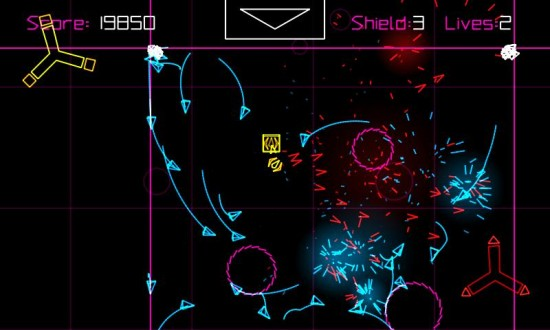
\includegraphics[width=0.75\textwidth]{4dd9c__pewpew-for-android-550x330.jpg}
\caption{Pandemonium game mode}
\end{figure}

\subsection*{Advisable criteria}
shield, lives, score, game controller, dual analog sticks, force feedback, adjustable camera perspective

\subsection*{Optional criteria}
second gun fire, special explosions, second kind of enemies, multiplayer, split screen

\subsection*{Demarcation criteria}
different levels, multiple game modes, ranking

\nocite{pewpewgame}
\nocite{iphoneappcafe}
\nocite{androidear}
\printbibliography

\listoffigures

\end{document}

